% This file defines the command for illustrating the conditional Gaussian distribution.
% It can be compiled standalone or included in a larger document.

\ifdefined\ispartofbook
\else
  % --- Standalone Compilation Preamble ---
  \documentclass[tikz, border=10pt]{standalone}
  \usepackage{tikz}
  \usetikzlibrary{arrows.meta, positioning, shapes.arrows}
  \begin{document}
\fi

% --- THE DIAGRAM COMMAND ---
\newcommand{\conditionalgaussiandiagram}{%
    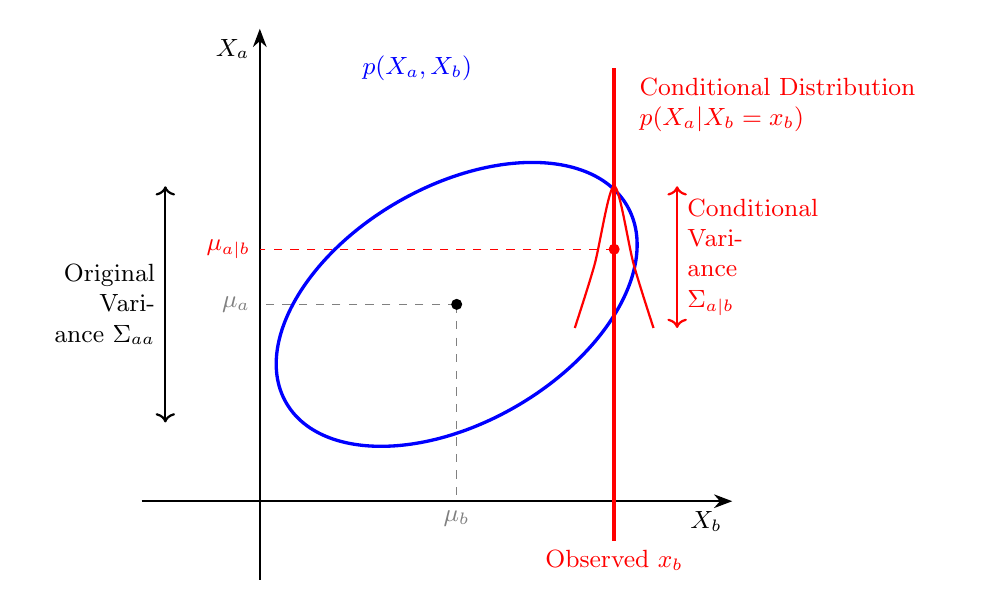
\begin{tikzpicture}[
        font=\sffamily,
        every node/.style={font=\small},
        arrow/.style={-Stealth, thick}
    ]
    % Axes
    \draw[-Stealth, thick] (-1.5,0) -- (6,0) node[below left] {$\vect{X}_b$};
    \draw[-Stealth, thick] (0,-1) -- (0,6) node[below left] {$\vect{X}_a$};

    % Joint Distribution Ellipse (representing a contour of p(Xa, Xb))
    \draw[blue, very thick, rotate around={30:(2.5,2.5)}] (2.5,2.5) ellipse (2.5cm and 1.5cm);
    \node[blue] at (2, 5.5) {$p(\vect{X}_a, \vect{X}_b)$};

    % Unconditional Means
    \draw[dashed, gray] (2.5,2.5) -- (2.5,0) node[below] {$\boldsymbol{\mu}_b$};
    \draw[dashed, gray] (2.5,2.5) -- (0,2.5) node[left] {$\boldsymbol{\mu}_a$};
    \fill[black] (2.5,2.5) circle (2pt);

    % Observation (the slice)
    \def\obsval{4.5}
    \draw[red, very thick] (\obsval, -0.5) -- (\obsval, 5.5);
    \node[red, below] at (\obsval, -0.5) {Observed $\vect{x}_b$};

    % Conditional Distribution p(Xa | Xb)
    \coordinate (slice_center) at (\obsval, 3.2); % Approximate center of the slice
    
    % Draw the 1D Gaussian bell curve for the conditional distribution
    \draw[red, thick, smooth] plot[domain=-1.5:1.5, samples=50] 
        coordinates {(\obsval-0.5, 3.2-1.0) (\obsval-0.25, 3.2-0.2) (\obsval, 3.2+0.8) (\obsval+0.25, 3.2-0.2) (\obsval+0.5, 3.2-1.0)};
    
    % Conditional Mean
    \draw[dashed, red] (slice_center) -- (0, 3.2) node[left] {$\boldsymbol{\mu}_{a|b}$};
    \fill[red] (slice_center) circle (2pt);
    
    % MODIFIED: Moved "Conditional Distribution..." text to be anchored to the left, just after the red line.
    \node[red, text width=4cm, align=left, anchor=north west] at (\obsval+0.2, 5.5)
        {Conditional Distribution $p(\vect{X}_a | \vect{X}_b=\vect{x}_b)$};

    % Illustrate variance reduction
    \draw[<->, thick, black] (-1.2, 1) -- (-1.2, 4) node[midway, left, text width=1.5cm, align=right] {Original Variance $\boldsymbol{\Sigma}_{aa}$};
    \draw[<->, thick, red] (\obsval+0.8, 2.2) -- (\obsval+0.8, 4.0) node[midway, right, text width=1cm] {Conditional Variance $\boldsymbol{\Sigma}_{a|b}$};

    \end{tikzpicture}%
}

\ifdefined\ispartofbook
  % This part is intentionally left blank when included in the main book.
\else
  % This part is for standalone compilation of the image.
  \conditionalgaussiandiagram
  \end{document}
\fi
